\documentclass[12pt,a4paper]{article}

%% ── Encoding & Fonts ─────────────────────────────────────────────────────────
\usepackage[T1]{fontenc}
\usepackage[utf8]{inputenc}
\usepackage{mathpazo}          % Palatino text + maths
\usepackage{microtype}         % better typography

%% ── Page Layout ─────────────────────────────────────────────────────────────
\usepackage[
  top=2.5cm, bottom=2.5cm,
  left=2.8cm, right=2.8cm,
  headheight=15pt
]{geometry}
\usepackage{setspace}
\onehalfspacing

%% ── Mathematics ─────────────────────────────────────────────────────────────
\usepackage{amsmath,amssymb,amsthm}

%% ── Tables ───────────────────────────────────────────────────────────────────
\usepackage{booktabs}
\usepackage{array}
\usepackage{multirow}
\usepackage{longtable}

%% ── Graphics & Colour ────────────────────────────────────────────────────────
\usepackage{graphicx}
\usepackage[dvipsnames,table]{xcolor}
\usepackage{tikz}
\usetikzlibrary{arrows.meta,positioning,shapes.geometric,calc}

%% ── Boxes ────────────────────────────────────────────────────────────────────
\usepackage[most]{tcolorbox}
\tcbuselibrary{breakable,skins}

%% ── Section Formatting ───────────────────────────────────────────────────────
\usepackage{titlesec}
\titleformat{\section}{\large\bfseries}{{\thesection.}}{0.6em}{}[\vspace{-2pt}\rule{\linewidth}{0.5pt}]
\titleformat{\subsection}{\normalsize\bfseries}{{\thesubsection}}{0.6em}{}
\titleformat{\subsubsection}{\normalsize\itshape}{{\thesubsubsection}}{0.6em}{}

%% ── Captions ─────────────────────────────────────────────────────────────────
\usepackage{caption}
\captionsetup{font=small,labelfont=bf,margin=1cm}

%% ── Lists ─────────────────────────────────────────────────────────────────────
\usepackage{enumitem}
\setlist[itemize]{noitemsep,topsep=4pt}
\setlist[enumerate]{noitemsep,topsep=4pt}

%% ── Headers & Footers ────────────────────────────────────────────────────────
\usepackage{fancyhdr}
\pagestyle{fancy}
\fancyhf{}
\fancyhead[L]{\small\textit{The Deposits Channel of Monetary Policy}}
\fancyhead[R]{\small\textit{Drechsler, Savov \& Schnabl (2017)}}
\fancyfoot[C]{\small\thepage}
\renewcommand{\headrulewidth}{0.4pt}

%% ── References ───────────────────────────────────────────────────────────────
\usepackage{natbib}
\bibliographystyle{aer}

%% ── Hyperlinks ───────────────────────────────────────────────────────────────
\usepackage[
  colorlinks=true,
  linkcolor=MidnightBlue,
  citecolor=MidnightBlue,
  urlcolor=MidnightBlue,
  bookmarks=true
]{hyperref}

%% ── Custom Colours ───────────────────────────────────────────────────────────
\definecolor{keyblue}{RGB}{0,63,114}
\definecolor{lightgray}{RGB}{245,245,245}
\definecolor{accentgold}{RGB}{180,140,0}
\definecolor{darkred}{RGB}{150,30,30}

%% ── Custom Environments ──────────────────────────────────────────────────────
\newtcolorbox{keybox}[1][Key Result]{
  enhanced, breakable,
  colback=keyblue!5!white,
  colframe=keyblue,
  fonttitle=\bfseries\small,
  title=#1,
  left=6pt, right=6pt,
  top=4pt, bottom=4pt,
  arc=3pt
}

\newtcolorbox{critbox}[1][Critical Assessment]{
  enhanced, breakable,
  colback=darkred!4!white,
  colframe=darkred!70!black,
  fonttitle=\bfseries\small,
  title=#1,
  left=6pt, right=6pt,
  top=4pt, bottom=4pt,
  arc=3pt
}

\newtcolorbox{extbox}[1][Extension]{
  enhanced, breakable,
  colback=accentgold!6!white,
  colframe=accentgold,
  fonttitle=\bfseries\small,
  title=#1,
  left=6pt, right=6pt,
  top=4pt, bottom=4pt,
  arc=3pt
}

%% ── Misc ──────────────────────────────────────────────────────────────────────
\usepackage{lipsum}
\usepackage{float}
\newcommand{\bps}{\,\text{bps}}
\newcommand{\FF}{\Delta FF}
\newcommand{\HHI}{\text{HHI}}
\newcommand{\R}{\mathbb{R}}

%% ─────────────────────────────────────────────────────────────────────────────
%%  DOCUMENT
%% ─────────────────────────────────────────────────────────────────────────────
\begin{document}

%% ── Title Page ───────────────────────────────────────────────────────────────
\begin{titlepage}
  \centering
  \vspace*{1.5cm}

  {\Large\bfseries\color{keyblue}
    The Deposits Channel of Monetary Policy}\\[0.5em]
  {\large A Comprehensive Critical Review}

  \vspace{1cm}
  \rule{0.5\linewidth}{0.8pt}
  \vspace{0.8cm}

  {\normalsize
    \textbf{Paper under review:}\\[0.3em]
    Drechsler, I., Savov, A., \& Schnabl, P. (2017).\\
    \textit{The Deposits Channel of Monetary Policy.}\\
    \textit{Quarterly Journal of Economics}, 132(4), 1819--1876.
  }

  \vspace{1.2cm}
  \rule{0.5\linewidth}{0.4pt}
  \vspace{0.8cm}

  {\small
  \begin{tabular}{ll}
    \textbf{Journal:} & \textit{Quarterly Journal of Economics}\\[3pt]
    \textbf{Volume / Issue:} & Vol.\ 132, No.\ 4, November 2017\\[3pt]
    \textbf{JEL Codes:} & E52, E58, G12, G21\\[3pt]
    \textbf{Review Date:} & April 2026\\
  \end{tabular}
  }

  \vfill

  \begin{tcolorbox}[
    colback=keyblue!8, colframe=keyblue,
    width=0.88\linewidth,
    arc=4pt, boxrule=0.6pt,
    fontupper=\small
  ]
  \textbf{Abstract.} This report provides a comprehensive critical review of
  Drechsler, Savov and Schnabl's (2017) seminal paper proposing the
  \emph{deposits channel} of monetary policy transmission. We examine the
  paper's theoretical framework, identification strategy, and empirical
  findings in depth; evaluate its strengths, limitations, and key
  assumptions; situate it within the broader monetary economics and banking
  literature; and propose substantive extensions relevant to the post-fintech
  era. We further assess the channel's contemporary relevance in light of the
  2022--2023 Federal Reserve tightening cycle, the collapse of Silicon Valley
  Bank, and the prospective introduction of central bank digital currencies.
  We conclude that the deposits channel constitutes one of the most important
  empirical and theoretical contributions to monetary economics of the past
  two decades, while identifying meaningful limitations that future research
  must address.
  \end{tcolorbox}

  \vspace{1cm}
\end{titlepage}

%% ── Table of Contents ────────────────────────────────────────────────────────
\tableofcontents
\newpage

%% ─────────────────────────────────────────────────────────────────────────────
\section{Introduction and Motivation}
%% ─────────────────────────────────────────────────────────────────────────────

The question of how monetary policy transmits through the banking system to
the real economy is one of the most consequential open problems in
macroeconomics. The prevailing theoretical framework --- the \emph{bank
lending channel} --- held that the Federal Reserve controlled the aggregate
supply of bank credit by regulating the quantity of required reserves. By
expanding or contracting reserves, the Fed could directly influence the size
of bank balance sheets and, through them, the volume of lending available to
households and firms \citep{bernanke_blinder_1988}.

This reserve mechanism, while theoretically clean, faced a fundamental
empirical obstacle: required reserves had become quantitatively negligible
relative to total bank assets by at least the 1980s. As documented by
\citet{romer_romer_1990}, \citet{bernanke_gertler_1995}, and
\citet{woodford_2010}, banks could easily circumvent reserve requirements by
adjusting the composition of their liabilities. The problem became acute
after 2008, when the Federal Reserve began paying interest on excess reserves,
making reserve requirements entirely non-binding in equilibrium. The bank
lending channel, in short, had compelling empirical support but no credible
theoretical foundation for the modern institutional environment.

\citet{dss2017} --- hereafter DSS --- fill this gap with a new mechanism: the
\textbf{deposits channel of monetary policy}. Their central claim is that banks
possess significant \emph{market power} over local deposit markets, and that
this market power --- rather than reserve requirements --- is the mechanism
through which changes in the Federal funds rate affect bank balance sheets and
ultimately the real economy.

The paper's central research question can be stated as follows: \emph{when
the Fed funds rate rises, how do banks adjust the spreads they charge on
deposits, how do depositors respond, and does the resulting funding contraction
translate into a reduction in bank lending and economic activity?}

The intuition is elegant. When the Fed funds rate is low, holding cash is
cheap, so households can easily substitute from deposits into cash. Banks must
therefore keep deposit spreads low to avoid losing their deposit base.
When the Fed funds rate rises, holding cash becomes expensive, which reduces
the sensitivity of depositors to deposit rates --- effectively granting banks
greater market power. Banks exploit this by widening spreads, and depositors
respond by gradually shifting into bonds and money market funds. Since deposits
are a uniquely stable and low-cost source of bank funding that cannot be
costlessly replaced by wholesale borrowing, the deposit contraction induces a
contraction in lending. DSS estimate this channel is large enough to account
for the \emph{entire} monetary policy transmission through bank balance sheets
documented in the prior empirical literature.

This review proceeds as follows. Section~\ref{sec:mechanism} develops the
economic intuition and theoretical framework. Section~\ref{sec:empirical}
describes the empirical strategy and identification approach.
Section~\ref{sec:results} summarises the main empirical findings.
Section~\ref{sec:critical} provides a detailed critical evaluation of the
paper's strengths and limitations. Section~\ref{sec:literature} situates DSS
within the broader literature. Section~\ref{sec:extensions} proposes
substantive extensions. Section~\ref{sec:contemporary} evaluates the channel's
contemporary relevance. Section~\ref{sec:conclusion} concludes.

%% ─────────────────────────────────────────────────────────────────────────────
\section{Economic Intuition and Theoretical Framework}
\label{sec:mechanism}
%% ─────────────────────────────────────────────────────────────────────────────

\subsection{The Core Transmission Mechanism}

The deposits channel operates through a sequence of interconnected steps that
link the Fed funds rate to real lending. Let $f$ denote the Fed funds rate and
$r_d$ the deposit rate. The \emph{deposit spread} is defined as $s \equiv f -
r_d$, representing the opportunity cost to depositors of holding deposits
rather than bonds. The core empirical regularity motivating DSS's theory is
that $s$ increases substantially when $f$ rises: for every 100 basis points
(bps) increase in the Fed funds rate, the aggregate deposit spread widens by
approximately 54\,bps. This \emph{incomplete pass-through} is the signature of
bank market power in the deposit market.

The mechanism linking the Fed funds rate to deposit spreads operates through
the outside option of depositors. Households derive liquidity from two main
instruments: cash (currency and zero-interest accounts) and deposits. Cash
provides maximal liquidity but pays no interest, so its opportunity cost equals
the Fed funds rate $f$. Deposits are less liquid than pure cash but pay a
positive rate $r_d = f - s$. Their opportunity cost relative to bonds is the
spread $s$.

When $f$ is low, cash is nearly costless to hold, making it a compelling
outside option. Depositors can cheaply substitute from deposits into cash,
so banks face highly elastic demand and must keep $s$ low. When $f$ is high,
cash becomes expensive to hold (its opportunity cost is $f$), so the relevant
outside option for depositors shifts from cash to bonds. Since bonds provide
no liquidity services and banks face limited within-market competition in
concentrated markets, deposit demand becomes more inelastic. Banks can therefore
widen $s$ without incurring proportionate outflows. The key insight is that
\textbf{bank market power is endogenous to the level of the Fed funds rate}.

\begin{keybox}[The Deposits Channel: Step-by-Step]
\begin{enumerate}
  \item $f \uparrow$ $\Rightarrow$ cost of holding cash rises
  \item Depositors less likely to substitute from deposits into cash
  \item Deposit demand becomes more inelastic; banks face less competition from cash
  \item Banks widen deposit spreads $s$ (keep $r_d$ low relative to $f$)
  \item Even though inelastic, depositors gradually shift to bonds/money markets
  \item Aggregate deposit outflows reduce banks' stable funding base
  \item Deposits cannot be fully replaced by costly wholesale funding
  \item Banks contract lending $\Rightarrow$ real economic activity falls
\end{enumerate}
\end{keybox}

\subsection{The Theoretical Model}

\subsubsection{Household Preferences}

The representative household maximises utility over final wealth $W$ and
liquidity services $l$ according to a constant elasticity of substitution
(CES) aggregator:
\begin{equation}
  u(W_0) = \max \left[ W^{\frac{\rho-1}{\rho}} + \lambda
  l^{\frac{\rho-1}{\rho}} \right]^{\frac{\rho}{\rho-1}},
  \label{eq:utility}
\end{equation}
where $\lambda > 0$ is a share parameter and $\rho < 1$ ensures that wealth
and liquidity are complements --- households value liquidity services
\emph{in addition to} financial returns, not as a substitute for them. This
preference structure is micro-founded either by a cash-in-advance constraint
\citep{gali_2009} or by a preference for extreme safety \citep{stein_2012}.

Liquidity services are themselves derived from cash $M$ and deposits $D$ via
a second CES aggregator:
\begin{equation}
  l(M, D) = \left[ M^{-\frac{1}{\epsilon}} + \delta
  D^{-\frac{1}{\epsilon}} \right]^{-\epsilon},
  \label{eq:liquidity}
\end{equation}
where $\epsilon > 1$ ensures cash and deposits are substitutes in the
provision of liquidity, and $\delta \in (0,1)$ captures the fact that deposits
are less liquid than cash. Deposits at different banks are themselves
imperfect substitutes, with elasticity of substitution $\eta > 1$ across
institutions, which gives individual banks market power.

\subsubsection{Equilibrium Deposit Spreads}

Each bank $i$ sets its deposit spread $s_i$ to maximise deposit profits
$D_i s_i$, subject to the household's demand system. In a symmetric
equilibrium with $N$ banks, the profit-maximising condition reduces to
equating the elasticity of demand for bank $i$'s deposits to $-1$. Solving
this optimality condition yields the equilibrium deposit spread:
\begin{equation}
  s = \delta^{\frac{1}{\epsilon-1}} \cdot
  \frac{\mathcal{M} - \rho}{\epsilon - \mathcal{M}} \cdot f,
  \label{eq:spread}
\end{equation}
where the market power parameter is:
\begin{equation}
  \mathcal{M} \equiv 1 - (\eta - 1)(N - 1).
  \label{eq:marketpower}
\end{equation}
Equation~\eqref{eq:marketpower} shows that market power $\mathcal{M}$ is
higher when there are fewer banks ($N$ small) or when depositors substitute
less readily across banks ($\eta$ close to 1). In the limiting case of a
monopolist, $\mathcal{M} = 1$.

From equation~\eqref{eq:spread}, three key theoretical predictions follow
directly:
\begin{enumerate}
  \item The deposit spread $s$ is \emph{proportional} to the Fed funds rate
    $f$, with factor:
    \[
      \frac{\mathcal{M}-\rho}{\epsilon-\mathcal{M}}\,
      \delta^{1/(\epsilon-1)}.
    \]
  \item The \emph{deposit spread beta}, defined as $\beta^s \equiv \partial s /
    \partial f$, is strictly increasing in market power $\mathcal{M}$.
  \item When $f$ is high, the aggregate elasticity of deposit demand approaches
    $\rho$ (the low wealth--liquidity substitution elasticity) because cash is
    expensive; when $f$ is low, it approaches $\epsilon$ (the higher
    cash--deposit substitution elasticity). Thus market power is endogenous to
    the rate level.
\end{enumerate}

\subsubsection{Financial Sophistication as an Additional Source of Market Power}

Geographic concentration is only one source of bank market power. DSS extend
the model (Proposition 2) to allow for a fraction $\alpha_{\text{ns}}$ of
``nonswitchers'' --- depositors who do not monitor rates at competing
institutions and therefore do not respond to spread differentials. The
equilibrium deposit spread beta is preserved in form, but with market power
parameter generalised to:
\begin{equation}
  \mathcal{M}_{\text{ns}} = 1 - (\eta-1)
  \left[ \frac{1}{\alpha_{\text{ns}} + (1-\alpha_{\text{ns}})\frac{1}{N}}
  - 1 \right]^{-1}.
  \label{eq:mns}
\end{equation}
This extension yields several important implications. First, the deposit spread
beta increases with the proportion of nonswitchers, as they represent an
additional source of insulated market power. Second, even in markets with zero
concentration (as $N \to \infty$), a sufficiently large fraction of
nonswitchers can sustain positive and economically meaningful spread betas.
Third, and most importantly, this result establishes that the deposit spread
beta is a \emph{sufficient statistic} for aggregate market power --- it
captures the combined effect of concentration, switching costs, financial
inattention, and depositor sophistication in a single observable metric.

\subsubsection{Effects on Lending and Wholesale Funding}

DSS extend the baseline model (Proposition 3) to incorporate profitable
lending opportunities (with decreasing marginal returns at rate $l_1$) and
costly wholesale (non-deposit) funding (with cost increasing at rate $h$).
Each bank $i$ now solves:
\begin{equation}
  \max_{D_i, H_i} \left[ f + l_0 - \frac{l_1}{2} L_i \right] L_i
  - \left[ f + \frac{h}{2} H_i \right] H_i - (f - s_i) D_i,
  \label{eq:bankproblem}
\end{equation}
where $L_i = H_i + D_i$ is total lending, $H_i$ is wholesale funding, and
$l_0, l_1, h > 0$.

The first-order condition for wholesale funding implies:
\begin{equation}
  H_i = \frac{l_0}{l_1 + h} - \frac{l_1}{l_1 + h} D_i.
  \label{eq:wholesale}
\end{equation}
Equation~\eqref{eq:wholesale} shows that banks partially offset a decline in
deposits by increasing wholesale funding. However, since wholesale funding is
costly ($h > 0$), this offset is only partial --- the Modigliani--Miller
theorem fails in this economy. Total lending is therefore:
\begin{equation}
  L_i = \frac{l_0}{l_1 + h} + \frac{h}{l_1 + h} D_i,
  \label{eq:lending}
\end{equation}
which is increasing in deposit volume. A contraction in deposits therefore
induces a contraction in lending, with magnitude governed by the ratio
$h/(l_1 + h)$. When $h$ is large (wholesale funding is very costly), the
pass-through from deposits to lending is near-complete; when $h$ is small,
banks can easily substitute and lending is relatively insulated.

Proposition 3 of DSS establishes that in this enriched model, all key
predictions from the baseline are preserved: higher rates increase the
effective market power of banks (raising $s$), inducing deposit contraction,
partial wholesale funding substitution, and a net reduction in lending.

%% ─────────────────────────────────────────────────────────────────────────────
\section{Empirical Strategy and Identification}
\label{sec:empirical}
%% ─────────────────────────────────────────────────────────────────────────────

\subsection{Data Sources}

DSS construct their empirical analysis from five primary datasets covering the
United States from 1994 to 2013:

\begin{itemize}
  \item \textbf{FDIC Summary of Deposits:} Annual branch-level deposit
    quantities for the universe of U.S. bank branches (June 1994--June 2014).
    Provides geographic coordinates, parent bank identifiers, and total deposit
    volumes.

  \item \textbf{Ratewatch:} Weekly branch-level deposit rates by product type,
    covering January 1997 to December 2013 and approximately 54\% of all U.S.
    bank branches. Focused analysis is on the two most widely-offered products:
    \$25,000 money market deposit accounts (savings proxy) and \$10,000
    12-month certificates of deposit (time deposit proxy).

  \item \textbf{U.S. Call Reports:} Quarterly bank-level income statements and
    balance sheets for all U.S. commercial banks (Federal Reserve Bank of
    Chicago, January 1994--December 2013).

  \item \textbf{NCRC Small Business Lending:} Annual new small business loan
    originations (loans $<$ \$1 million) at the bank-county level from 1997 to
    2013.

  \item \textbf{FRED and Datastream:} Fed funds target rate, one-year T-bill
    rate, and Fed funds futures prices for expected-rate decomposition.
\end{itemize}

Market concentration is measured using the Herfindahl-Hirschman Index
(\HHI), defined for county $c$ in year $t$ as:
\begin{equation}
  \HHI_{ct} = \sum_{j=1}^{N_{ct}} \left( \frac{D_{jct}}{D_{ct}} \right)^2,
  \label{eq:hhi}
\end{equation}
where $D_{jct}$ is bank $j$'s deposits in county $c$ at time $t$, and
$D_{ct}$ is total county deposits. Branch-\HHI\ is the time-averaged value
of equation~\eqref{eq:hhi} for the county where a branch is located.
Bank-\HHI\ is the deposit-weighted average of Branch-\HHI\ across all of a
bank's branches.

The resulting cross-sectional variation is substantial. Branch-\HHI\ ranges
from 0.06 in the most competitive urban markets to 1.0 in monopolistic rural
counties, with a mean of 0.35 and standard deviation of 0.20 across counties.

\subsection{The Identification Challenge}

The central identification problem is that deposit supply and banks' lending
opportunities may be simultaneously affected by macroeconomic conditions. When
the Fed raises rates in response to an economic expansion, loan demand may
also be elevated, causing banks to take in more deposits independently of any
deposit channel. Conversely, if tightening accompanies a downturn, declining
loan demand may reduce deposit-taking even in the absence of market power
effects. A simple time-series regression of deposit growth on the Fed funds
rate cannot disentangle these supply and demand effects.

\subsection{Within-Bank, Across-Branch Estimation}

DSS's primary solution is a within-bank, across-branch identification strategy
that exploits geographic variation in deposit market concentration. The
fundamental observation is that since banks operate internal capital markets
--- raising deposits at some branches and lending them at others --- the
deposit decision at a given branch is separable from local lending decisions.
By comparing branches of the \emph{same bank} located in counties with
\emph{different} \HHI\ levels, DSS can control for the bank's lending
opportunities while estimating the pure market power effect.

The baseline panel regression is:
\begin{equation}
  \Delta y_{it} = \alpha_i + \zeta_{c(i)} + \lambda_{s(i)t}
  + \delta_{j(i)t} + \gamma \cdot \Delta FF_t
  \times \text{Branch-HHI}_i + \varepsilon_{it},
  \label{eq:main_reg}
\end{equation}
where:
\begin{itemize}
  \item $\Delta y_{it}$ is either the change in the deposit spread or the log
    change in total deposits at branch $i$ from $t$ to $t+1$;
  \item $\Delta FF_t$ is the contemporaneous change in the Fed funds target
    rate;
  \item $\text{Branch-HHI}_i$ is the time-averaged \HHI\ of the county where
    branch $i$ is located;
  \item $\delta_{j(i)t}$ are \textbf{bank $\times$ time fixed effects} for the
    bank $j$ that owns branch $i$ --- the key control that absorbs all
    time-varying bank-specific factors, including lending opportunities;
  \item $\alpha_i$, $\zeta_{c(i)}$, and $\lambda_{s(i)t}$ are branch, county,
    and state$\times$time fixed effects, respectively;
  \item Standard errors are clustered at the county level.
\end{itemize}

The coefficient of interest is $\gamma$: the differential sensitivity of
deposit spreads (or flows) to monetary policy, as a function of local market
concentration. The identifying assumption is that banks equalise marginal
returns to lending across their branches, so that the deposit allocation
decision at each branch is independent of local lending conditions. This
assumption is supported by the within-county lending results in Section 7 of
DSS, which show that a bank's lending in a given county is unrelated to the
local concentration of deposit markets (supporting internal fund allocation),
and by external evidence from \citet{gilje_loutskina_strahan_2016} showing
that banks channel deposits toward high-demand lending markets.

\subsection{Event Study: Timing of Deposit Spread Adjustment}

To provide sharper causal identification, DSS exploit the weekly frequency of
Ratewatch data to conduct an event study around FOMC announcements. The
regression is:
\begin{equation}
  \Delta y_{it} = \alpha_t + \zeta_{c(i)} + \sum_{\tau=-5}^{5}
  \gamma_\tau \cdot \text{Branch-HHI}_{c(i)} \times \Delta FF_{t-\tau}
  + \varepsilon_{it},
  \label{eq:event_study}
\end{equation}
where the five leads and lags of $\Delta FF$ encompass the full six-week FOMC
decision cycle. The cumulative sum $\sum_{\tau=-5}^{t} \gamma_\tau$ traces
the differential spread response at high- versus low-concentration branches
around week 0 (the announcement week).

If the deposits channel is the true mechanism, we expect: (i) no differential
pre-announcement drift (ruling out anticipation effects); (ii) a sharp
response beginning in week 0 (consistent with a direct monetary policy
effect); and (iii) a permanent level shift thereafter (consistent with the
quarterly regression magnitudes).

\subsection{Decomposition into Expected and Unexpected Rate Changes}

A further identification test exploits the fact that savings deposits have
zero maturity, so their rates should respond to a rate change \emph{when it
occurs} regardless of whether it was anticipated. This contrasts with long-lived
assets like stocks and bonds, which incorporate expected rate changes in advance
and react only to surprises. DSS replace the total rate change in
equation~\eqref{eq:main_reg} with its expected component (measured from Fed
funds futures prices three months prior) and the unexpected residual, finding
that both components have quantitatively similar effects on deposit spreads.
This decomposition rules out the interpretation that the results are driven by
information released at the time of FOMC decisions rather than by the rate
change itself.

\subsection{Lending Channel Identification: Within-County Estimation}

For the lending analysis, banks can allocate deposits across branches, so the
within-bank identification strategy used for deposits is inapplicable. Instead,
DSS compare the lending behaviour of different banks within the same county
(same lending market) while varying their bank-level deposit concentration
(Bank-\HHI). The lending regression is:
\begin{equation}
  \Delta \log(\text{lending})_{jct} = \alpha_{jc} + \delta_{ct}
  + \beta \cdot \text{Bank-HHI}_{jt-1}
  + \gamma \cdot \Delta FF_t \times \text{Bank-HHI}_{jt-1}
  + \varepsilon_{jct},
  \label{eq:lending_reg}
\end{equation}
where $\alpha_{jc}$ are bank$\times$county fixed effects and $\delta_{ct}$ are
county$\times$time fixed effects that absorb all local lending demand changes.
The coefficient $\gamma$ identifies whether, controlling for local demand,
banks with more concentrated deposit bases (higher Bank-\HHI) reduce lending
more when the Fed funds rate rises.

%% ─────────────────────────────────────────────────────────────────────────────
\section{Key Empirical Findings}
\label{sec:results}
%% ─────────────────────────────────────────────────────────────────────────────

\subsection{Aggregate Time-Series Evidence}

The aggregate time series provides compelling prima facie evidence for the
deposits channel. Figure~I of DSS plots the average deposit rate against the
Fed funds target rate from 1986 to 2013, revealing a striking pattern of
incomplete pass-through: deposit rates consistently track the Fed funds rate,
but with a systematic lag and shortfall.

\begin{keybox}[Aggregate Spread Evidence]
For every 100\,bps increase in the Fed funds rate, the aggregate deposit spread
widens by \textbf{54\,bps}. During the 425\,bps mid-2000s hiking cycle, the
deposit spread rose by 245\,bps. Spreads on savings and checking deposits
increased by 340\,bps and 470\,bps respectively, while time deposit spreads
rose by only 105\,bps --- consistent with greater market power over more liquid
deposit categories.
\end{keybox}

Figure~II of DSS documents deposit quantity responses. Core deposit growth is
strongly negatively correlated with changes in the Fed funds rate (correlation
$= -49\%$), with year-over-year growth rates ranging from $-1\%$ to $+18\%$
over the sample. The correlations are stronger for liquid categories (savings:
$-59\%$, checking: $-33\%$) and positive for illiquid time deposits ($+23\%$),
reflecting within-deposit substitution as liquid instruments become relatively
more expensive.

Crucially, the simultaneous observation of rising spreads and falling deposit
quantities identifies a \emph{supply curve shift}: if the effect were driven
by a demand shift, prices and quantities would move in the same direction.

\subsection{Branch-Level Within-Bank Results}

Table~\ref{tab:spread_results} summarises the within-bank estimation results
from equations~\eqref{eq:main_reg} for deposit spreads and flows.

\begin{table}[H]
\centering
\caption{Deposit Spreads, Flows, and Monetary Policy: Within-Bank Estimates}
\label{tab:spread_results}
\small
\begin{tabular}{lcccc}
\toprule
 & \multicolumn{2}{c}{\textbf{Spread Response}} &
   \multicolumn{2}{c}{\textbf{Flow Response}} \\
\cmidrule(lr){2-3}\cmidrule(lr){4-5}
 & Savings & Time & & \\
\textbf{Specification} & $\Delta\text{Spread}$ & $\Delta\text{Spread}$ &
  \multicolumn{2}{c}{$\Delta\log(\text{Deposits})$} \\
\midrule
$\Delta FF \times \text{Branch-HHI}$
  & $0.140^{***}$ & $0.074^{***}$ & $-0.661^{***}$ & \\
  & $(0.033)$ & $(0.025)$ & $(0.254)$ & \\[4pt]
Bank $\times$ Quarter FE & \checkmark & \checkmark & \checkmark & \\
State $\times$ Quarter FE & \checkmark & \checkmark & \checkmark & \\
Branch FE & \checkmark & \checkmark & \checkmark & \\
County FE & \checkmark & \checkmark & \checkmark & \\
Observations & 117,683 & 121,990 & 1,150,049 & \\
$R^2$ & 0.810 & 0.808 & 0.344 & \\
\bottomrule
\end{tabular}

\vspace{4pt}
\footnotesize
\textit{Notes.} Standard errors clustered at county level in parentheses.
$^{***}$ $p<0.01$, $^{**}$ $p<0.05$, $^*$ $p<0.1$. Preferred specification
with full set of fixed effects shown. Source: DSS (2017), Tables II and III.
\end{table}

Following a 100\,bps increase in the Fed funds rate, branches of the same bank
in high-concentration counties raise savings deposit spreads by \textbf{14\,bps
more} and experience deposit outflows \textbf{66\,bps larger} than branches in
low-concentration counties. The results are robust across all specification
variants, including with and without state$\times$time fixed effects.

The implied semi-elasticity of deposits with respect to deposit spreads is
$-5.3$, meaning a 100\,bps increase in the deposit spread is associated with a
530\,bps contraction in deposits. Since a 100\,bps rate hike generates on
average a 61\,bps spread increase among large banks, the implied deposit
contraction per 100\,bps hike is approximately 323\,bps.

\subsection{Event Study Results}

Figure~V of DSS (reproduced schematically as Figure~\ref{fig:event_study_tikz}
below) provides some of the most compelling evidence in the paper.

\begin{figure}[H]
\centering
\resizebox{\linewidth}{!}{%
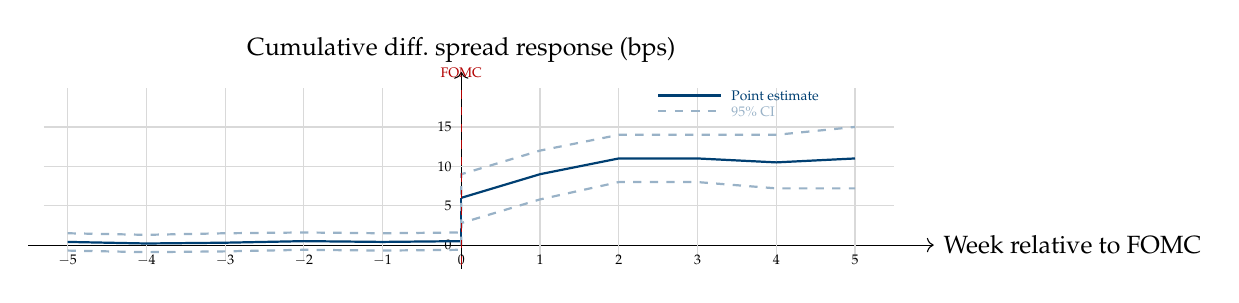
\begin{tikzpicture}[scale=1.0]
  % Axes
  \draw[->] (-5.5,0) -- (6,0) node[right]{\small Week relative to FOMC};
  \draw[->] (0,-0.3) -- (0,2.2) node[above]{\small Cumulative diff.\ spread response (bps)};

  % Grid
  \foreach \x in {-5,-4,-3,-2,-1,1,2,3,4,5}
    \draw[gray!30] (\x,-0.2) -- (\x,2.0);
  \foreach \y in {0.5,1.0,1.5}
    \draw[gray!30] (-5.3,\y) -- (5.5,\y);

  % Tick labels
  \foreach \x in {-5,-4,-3,-2,-1,0,1,2,3,4,5}
    \node[below,font=\tiny] at (\x,0) {$\x$};
  \foreach \y/\lab in {0/0, 0.5/5, 1.0/10, 1.5/15}
    \node[left,font=\tiny] at (0,\y) {\lab};

  % Pre-announcement: flat near zero
  \draw[keyblue,thick] (-5,0.04) -- (-4,0.02) -- (-3,0.03)
    -- (-2,0.05) -- (-1,0.04) -- (0,0.05);

  % Jump at announcement
  \draw[keyblue,thick] (0,0.05) -- (0,0.6);
  \draw[keyblue,thick] (0,0.6) -- (1,0.9) -- (2,1.1) -- (3,1.1)
    -- (4,1.05) -- (5,1.1);

  % Confidence band (dashed)
  \draw[keyblue!40,dashed,thick] (-5,0.15) -- (-4,0.13) -- (-3,0.15)
    -- (-2,0.16) -- (-1,0.15) -- (0,0.16)
    -- (0,0.9) -- (1,1.2) -- (2,1.4) -- (3,1.4) -- (4,1.4) -- (5,1.5);
  \draw[keyblue!40,dashed,thick] (-5,-0.07) -- (-4,-0.09) -- (-3,-0.08)
    -- (-2,-0.06) -- (-1,-0.07) -- (0,-0.06)
    -- (0,0.28) -- (1,0.58) -- (2,0.8) -- (3,0.8) -- (4,0.72) -- (5,0.72);

  % FOMC announcement marker
  \draw[red!70!black, dashed] (0,-0.25) -- (0,2.0)
    node[above,font=\tiny,red!70!black]{FOMC};

  % Legend
  \draw[keyblue,thick] (2.5,1.9) -- (3.3,1.9)
    node[right,font=\tiny]{Point estimate};
  \draw[keyblue!40,dashed,thick] (2.5,1.7) -- (3.3,1.7)
    node[right,font=\tiny]{95\% CI};
\end{tikzpicture}%
}
\captionsetup{justification=raggedright,singlelinecheck=false}
\caption{Event-study differential deposit spread response (DSS, Figure~V).}
\label{fig:event_study_tikz}
\end{figure}

The event study confirms: (i) zero differential pre-announcement response,
ruling out anticipation and slow-moving confounds; (ii) a jump of approximately
6\,bps in the week of the FOMC decision; (iii) accumulation to $\approx 11$\,bps
over the following two weeks; and (iv) a permanent level shift consistent with
the quarterly regression estimates.

\subsection{Financial Sophistication}

Table~V of DSS confirms that financial sophistication amplifies market power
independently of concentration. Using county-level proxies --- share of
population aged 65+ (age), log median household income (income), and share
with a college degree (education) --- DSS find that branches in counties with
older, lower-income, or less-educated populations raise spreads more and
experience greater outflows when rates rise, all else equal. College education
is the most robust proxy when all three are included jointly. These findings
validate Proposition~2: the deposit spread beta is a sufficient statistic for
market power from both structural (concentration) and behavioral (sophistication)
sources.

\subsection{Lending and Real Economic Activity}

\begin{table}[H]
\centering
\caption{Deposits Channel Effects on Lending and Real Activity}
\label{tab:lending_results}
\small
\begin{tabular}{lcc}
\toprule
\textbf{Outcome} & \textbf{Coefficient} & \textbf{Significance} \\
\midrule
\multicolumn{3}{l}{\textit{Bank-county lending (within-county estimation)}} \\
$\Delta FF \times \text{Bank-HHI}$ (new SB lending) & $-0.208$ per unit HHI & $**$ \\
$\quad$ Per 1 SD increase in Bank-HHI & $-291$\,bps per 100\,bps hike & $**$ \\[6pt]
\multicolumn{3}{l}{\textit{County-level outcomes (within-county estimation)}} \\
$\Delta FF \times \text{County-HHI}$ (new lending) & $-0.093$ & $***$ \\
$\quad$ Per 1 SD increase (58\,bps per 100\,bps) & & \\
$\Delta FF \times \text{County-HHI}$ (employment $\Delta$) & $-0.014$ & $***$ \\
$\quad$ Per 1 SD increase ($-9$\,bps per 100\,bps) & & \\
$\Delta FF \times \text{County-HHI}$ (wage bill $\Delta$) & $-0.011$ & $***$ \\
$\quad$ Per 1 SD increase ($-11$\,bps per 100\,bps) & & \\
\bottomrule
\end{tabular}

\vspace{4pt}
\footnotesize
\textit{Notes.} $^{***}$ $p<0.01$, $^{**}$ $p<0.05$. SB = small business.
Standard errors double-clustered at bank and county level (lending regressions)
or clustered at county level (county-level regressions). Source: DSS (2017),
Tables VI and VII.
\end{table}

Table~\ref{tab:lending_results} shows that the deposit contraction has
economically and statistically significant effects on lending and employment.
Small business lending is particularly sensitive because it is illiquid and
risky, making it highly dependent on the stable funding that deposits uniquely
provide.

The bank-level Call Reports analysis (Table~VIII of DSS) corroborates these
findings. Banks with higher Bank-\HHI\ experience greater deposit outflows,
partially offset by increased wholesale funding, with a net contraction in
total liabilities. Assets decline correspondingly, driven by reductions in
securities, real estate loans, and commercial and industrial loans.

\subsection{Aggregate Scale and the Deposit Spread Beta}

The deposit spread beta, estimated by regressing each bank's deposit spread on
the Fed funds rate (with up to four lags to allow for adjustment in
non-zero-maturity products), averages 0.54 across all banks and 0.61 for the
largest 5\% of banks. The cross-sectional distribution is wide, ranging from
0.31 at the 10th percentile to 0.89 at the 90th percentile.

\begin{keybox}[Aggregate Quantitative Implications]
\small
\begin{center}
\begin{tabular}{p{6.6cm}cc}
\toprule
\textbf{Outcome (400\,bps hiking cycle)} & \textbf{Percentage} &
  \textbf{Dollar value (2014 base)} \\
\midrule
Deposit reduction & $-1{,}458$\,bps & \textbf{\$1.35 trillion} \\
Lending reduction & $-995$\,bps & \textbf{\$763 billion} \\
\midrule
\multicolumn{3}{p{10.6cm}}{\textit{Comparison to Bernanke \& Blinder (1992)
VAR (per 31\,bps hike):}} \\
Deposit outflows: B\&B = 81\,bps; DSS = 113\,bps & & \\
Securities reduction: B\&B = 123\,bps; DSS = 154\,bps & & \\
Loan contraction: B\&B = 57\,bps; DSS = 77\,bps & & \\
\bottomrule
\end{tabular}
\end{center}
\smallskip
DSS estimates are large enough to account for the \emph{entire} transmission
of monetary policy through bank balance sheets documented in the prior
literature --- without requiring any role for reserve requirements.
\end{keybox}

\subsection{The Liquidity Premium}

Since deposits are the primary source of liquid assets for households, their
contraction mechanically reduces the aggregate supply of liquidity in the
economy. DSS document a striking 90\% correlation between the aggregate deposit
spread and the T-bill liquidity premium (defined as the Fed funds rate minus
the three-month T-bill rate) over 1986--2013. This relationship is strong both
at business cycle frequencies and in long-run trends.

This finding connects the deposits channel to the broader asset pricing
literature. When monetary policy tightens and deposit spreads widen, the supply
of household liquidity contracts, pushing up the liquidity premium on all safe
and liquid assets including Treasury securities. This provides a supply-side
explanation for the puzzling tight relationship between the Fed funds rate and
the liquidity premium documented by \citet{nagel_2016}, which had previously
lacked a micro-founded theoretical account.

%% ─────────────────────────────────────────────────────────────────────────────
\section{Critical Evaluation}
\label{sec:critical}
%% ─────────────────────────────────────────────────────────────────────────────

\subsection{Strengths}

\subsubsection{Identification Strategy}

The within-bank, across-branch design is among the most credible natural
experiments in the empirical banking literature. By holding the bank fixed
(through bank$\times$time fixed effects) and exploiting plausibly exogenous
geographic variation in market concentration, DSS cleanly isolate the market
power mechanism from the confounding effect of lending opportunities. The
event study's week-zero timing response closes off virtually all remaining
alternative explanations. These two identification strategies are mutually
reinforcing rather than redundant: the quarterly panel regression establishes
the magnitude and persistence of the concentration effect, while the event
study pins down precise causal timing.

\subsubsection{Empirical Breadth and Internal Consistency}

Results are consistent across five levels of analysis --- aggregate time series,
branch-level spread and flow regressions, bank-level Call Reports, county-level
employment outcomes, and the event study around FOMC announcements --- using
three independent datasets (Ratewatch, FDIC, Call Reports). Quantitative
magnitudes are also internally consistent: the within-bank semi-elasticity
($-5.3$) and the spread-beta-based estimate ($-3.6$ for all banks, $-6.0$ for
large banks) bracket a plausible range, and both align with the aggregate
time-series patterns. This multi-level consistency is a powerful indicator
of a genuine mechanism rather than a statistical artefact.

\subsubsection{The Deposit Spread Beta as a Policy Instrument}

The deposit spread beta is a theoretically grounded, easily observable,
bank-level measure of monetary policy exposure that aggregates all sources of
market power --- concentration, switching costs, financial sophistication,
product differentiation --- into a single sufficient statistic. This has
genuine practical value for bank supervisors and macroprudential regulators
seeking to identify which institutions are most exposed to rate cycles. It
also provides a natural metric for stress testing: a bank with a high spread
beta will experience larger deposit outflows and greater balance sheet
contraction for a given tightening episode.

\subsubsection{Resolution of a Long-Standing Theoretical Puzzle}

By providing a market-power foundation for the bank lending channel, DSS
resolve a problem that had persisted in monetary economics for over three
decades. The mechanism requires no reserves, no binding capital constraints,
and no assumption about long-term rate movements --- it operates through the
level of the short rate, which is precisely the instrument the Fed controls.
This also provides theoretical grounding for the observed practice of gradual
rate adjustment, since each rate change has a direct and meaningful effect on
deposit supply independent of its level relative to the natural rate.

\subsection{Weaknesses and Limitations}

\begin{critbox}[Representative Household Assumption]
The CES framework aggregates all depositors into a single representative agent
with constant elasticity preferences. This fundamentally cannot capture the
heterogeneity in depositor behaviour that drives the tail risks most relevant
to financial stability. Wealthy, financially sophisticated depositors ---
corporate treasurers, institutional cash managers, and high-net-worth
individuals --- have near-zero switching costs and near-infinite elasticity.
Retail depositors exhibit high inertia, inattention, and genuine switching
costs. Aggregating these populations produces average parameters that may
accurately predict gradual, economy-wide adjustment while completely missing
the concentrated, rapid outflows that precipitate bank runs. The Silicon
Valley Bank episode (Section~\ref{sec:contemporary}) illustrates precisely
this limitation.
\end{critbox}

\begin{critbox}[Pre-Fintech Sample Period: 1994--2013]
The empirical analysis predates the structural disruption of digital banking.
The rise of online high-yield savings accounts (e.g., Marcus by Goldman Sachs,
Ally Bank), mobile banking applications, and fintech platforms from
approximately 2015 onward has dramatically reduced geographic switching
frictions. A depositor in 2024 can open a new account in minutes on a
smartphone, rendering county-level \HHI\ a less meaningful proxy for
competitive pressure than it was in 2005. The model's market power parameters
--- and therefore its quantitative predictions for the magnitude and speed of
the deposits channel --- likely require substantial re-estimation for the
post-2015 era. The 2022--2023 hiking cycle, discussed in
Section~\ref{sec:contemporary}, provides preliminary evidence of faster
adjustment consistent with reduced switching costs.
\end{critbox}

\begin{critbox}[Wholesale Funding Cost: Assumed Rather Than Estimated]
The parameter $h$ governing the marginal cost of wholesale funding plays a
central role in translating deposit outflows into lending contraction
(equation~\ref{eq:lending}), but is not directly estimated. In practice, this
cost varies substantially with macroeconomic conditions, a bank's credit
rating, the regulatory environment (Basel III's Liquidity Coverage Ratio and
Net Stable Funding Ratio impose explicit costs on wholesale reliance), and
prevailing stress in money markets. Treating $h$ as a fixed structural constant
limits the model's portability across different regulatory regimes and time
periods, and introduces unquantified sensitivity in the lending contraction
estimates.
\end{critbox}

\begin{critbox}[Static and Geographic Concentration Measure]
Branch-\HHI\ is computed as a time-averaged, county-level measure that
abstracts from dynamic competitive entry, the growing role of non-bank
competitors (money market funds, brokerage platforms, fintech lenders), and
cross-geographic competition from internet banks. In the modern era, a bank's
true competitive environment in deposit-taking is increasingly defined by
product characteristics and digital accessibility rather than geographic
proximity. The assumption that county-level \HHI\ adequately proxies for a
bank's market power becomes increasingly tenuous as the share of online
deposit-taking grows.
\end{critbox}

\begin{critbox}[General Equilibrium and Endogeneity of Aggregate Estimates]
DSS acknowledge that because the Fed tends to raise rates during economic
expansions, aggregate lending at the time of a hiking cycle is elevated by
high loan demand, partially offsetting the deposit-channel-induced contraction.
The cross-sectional identification controls for this at the bank and county
level, but the aggregate dollar estimates (\$1.35T deposits, \$763B lending)
are necessarily computed under the counterfactual assumption that lending would
have remained unchanged. These are therefore best interpreted as upper bounds
on the net contractionary effect of a tightening cycle.
\end{critbox}

\subsection{Assessment of Key Assumptions}

\begin{table}[H]
\centering
\caption{Assessment of Core Modelling and Identification Assumptions}
\label{tab:assumptions}
\small
\begin{tabular}{@{}p{4.6cm} p{3.6cm} p{5.2cm}@{}}
\toprule
\textbf{Assumption} & \textbf{Role in Paper} & \textbf{Assessment} \\
\midrule
Banks freely allocate deposits across branches &
  Enables within-bank identification &
  Indirectly validated by lending regressions; may fail for small
  single-market banks ($\sim$30\% of sample) \\[6pt]

Wealth and liquidity are complements ($\rho < 1$) &
  Drives demand inelasticity at high rates &
  Well-grounded in cash-in-advance and safety-preference frameworks;
  validated by liquid vs.\ illiquid deposit differential \\[6pt]

Cash and deposits are substitutes ($\epsilon > 1$) &
  Ensures households switch to cash when rates are low &
  Consistent with near-zero cash demand at low rates in equilibrium \\[6pt]

Market power stable over time &
  Justifies time-averaged \HHI\ measure &
  Increasingly tenuous post-2015; digital banking disrupts
  geographic concentration \\[6pt]

Wholesale funding cost $h$ is constant &
  Governs lending channel magnitude &
  Varies with regulation, stress, and monetary regime; not estimated \\[6pt]

Representative household &
  Enables clean aggregation &
  Problematic for heterogeneous depositor dynamics and tail risk
  (SVB, bank runs) \\
\bottomrule
\end{tabular}
\end{table}

%% ─────────────────────────────────────────────────────────────────────────────
\section{Engagement with the Broader Literature}
\label{sec:literature}
%% ─────────────────────────────────────────────────────────────────────────────

\subsection{The Bank Lending Channel}

The deposits channel directly addresses the long-standing theoretical gap in
the bank lending channel literature initiated by \citet{bernanke_blinder_1988}
and elaborated by \citet{kashyap_stein_1994}, \citet{kashyap_stein_wilcox_1993},
and \citet{kashyap_stein_2000}. These papers documented robust empirical
relationships between monetary policy and bank credit supply but relied on
reserve requirements as the transmission mechanism --- a foundation that had
become implausible by the 1990s. DSS provide the new micro-foundation the
literature needed. Quantitatively, their estimates bracket the VAR-based
estimates of \citet{bernanke_blinder_1992}, with their aggregate figures
accounting for the full magnitude of bank balance sheet transmission.

\subsection{The Balance Sheet Channel}

The deposits channel makes a sharply different prediction from the balance
sheet or net worth channel of \citet{bernanke_gertler_1989},
\citet{kiyotaki_moore_1997}, and \citet{brunnermeier_sannikov_2014}. Under
balance sheet amplification, a surprise increase in long-term interest rates
reduces bank net worth, forcing a symmetric contraction in all liabilities.
Under the deposits channel, banks specifically \emph{reduce deposit funding
and increase wholesale funding} --- a substitution that is consistent with
what DSS observe empirically. This differential prediction provides clean
discriminating power between the two channels.

\subsection{The New Keynesian Framework}

DSS complement rather than replace the New Keynesian model \citep{woodford_2003},
but with two important distinctions. In the standard New Keynesian framework,
the short rate matters only insofar as it influences long-term rates through
the expectations hypothesis. In the deposits channel, the short rate matters
\emph{in its own right} because it directly affects the supply of liquid assets
and the cost of bank funding. This provides a theoretical basis for the
empirical observation that the level of the short rate --- not just its
deviation from the neutral rate --- influences economic outcomes, and for the
practice of gradual rate adjustment \citep{bernanke_2004, stein_sunderam_2015}.

\subsection{Deposit Pricing and Market Structure}

The deposit pricing literature \citep{hannan_berger_1989, hannan_berger_1991,
neumark_sharpe_1992, driscoll_judson_2013} documents that deposit rate
adjustment is slow and asymmetric, particularly in concentrated markets, and
interprets this as evidence of New Keynesian price rigidities. DSS depart from
this interpretation in two important ways: they focus on permanent changes in
the \emph{level} of deposit spreads (not the adjustment speed), and they
jointly analyse deposit quantities, which prior work largely ignored. This
joint analysis of prices and quantities is essential for identifying supply
versus demand effects and for quantifying the aggregate implications of the
channel.

\subsection{The Liquidity Premium Literature}

\citet{nagel_2016} documents a puzzling 90\% correlation between the Fed funds
rate and the T-bill liquidity premium over several decades, but does not
provide a micro-founded supply-side explanation. DSS fill this gap: by showing
that deposit supply contracts when rates rise, they explain how monetary policy
mechanically reduces aggregate household liquidity and pushes up the liquidity
premium on all safe assets. This connects monetary economics to the asset
pricing literature on the convenience yield of near-money assets
\citep{krishnamurthy_vissing_2012}, suggesting that monetary transmission
operates not just through credit supply but through liquidity pricing across
all financial markets.

%% ─────────────────────────────────────────────────────────────────────────────
\section{Extensions and Avenues for Future Research}
\label{sec:extensions}
%% ─────────────────────────────────────────────────────────────────────────────

\begin{extbox}[Extension 1: Digital Banking and the Structural Erosion of Market Power]
\textbf{Hypothesis.} The rise of online high-yield savings platforms and mobile
banking from $\sim$2015 onward has structurally reduced geographic switching
frictions, compressing deposit spread betas toward zero.

\textbf{Empirical design.} Exploit the staggered geographic rollout of major
online savings products (e.g., Marcus by Goldman Sachs, launched 2016; Ally
Bank's mobile app penetration) as a quasi-exogenous shock to the competitive
environment faced by incumbent brick-and-mortar banks. Estimate whether spread
betas and the sensitivity of deposit outflows to rate changes declined
following exposure to online bank entry. Use county-level smartphone adoption
rates and broadband penetration as instrumental variables for the timing of
digital banking disruption.

\textbf{Expected finding.} Spread betas should have declined monotonically
with digital bank market share, particularly in previously high-\HHI\
counties where the disruption was most pronounced. If confirmed, this implies
that the deposits channel has been weakening as a monetary transmission
mechanism precisely as the Fed has become more reliant on rate-based policy ---
with potential implications for the size and duration of rate cycles required
to achieve a given macroeconomic effect.
\end{extbox}

\begin{extbox}[Extension 2: Central Bank Digital Currency and the Deposit Channel]
A retail CBDC paying a rate mechanically linked to monetary policy would
constitute direct government competition with bank deposits. This creates
fundamentally opposing forces for the deposits channel.

\textbf{Amplification effect.} With a CBDC available at zero switching cost
and government backing, depositors would immediately and fully substitute out
of bank deposits when rates rise and the CBDC rate adjusts instantaneously.
Pass-through would approach unity, accelerating and intensifying the deposit
channel's operation.

\textbf{Destruction effect.} The existence of the CBDC as a permanent outside
option would eliminate banks' market power in deposit markets entirely ---
driving spread betas toward zero in steady state, collapsing deposit franchise
values, and potentially triggering systematic bank disintermediation.

\textbf{Model extension.} Introduce the CBDC as a fourth asset class in the
household's liquidity aggregator (equation~\ref{eq:liquidity}), paying rate
$r_{\text{CBDC}} = f - s_{\text{CBDC}}$ where $s_{\text{CBDC}}$ is a small
fixed spread set by the central bank. Solve for equilibrium bank spreads and
deposit quantities as a function of CBDC adoption rates. Quantify the tradeoff
between faster policy transmission and the financial stability risk of rapid
bank disintermediation during tightening cycles.
\end{extbox}

\begin{extbox}[Extension 3: Heterogeneous Depositor Model]
Replace the representative household in equations~\eqref{eq:utility}--
\eqref{eq:liquidity} with a distribution of depositor types indexed by
sophistication parameter $\theta_i \sim F(\theta)$, where $\theta_i$ governs
both switching costs and awareness of competing rates.

\textbf{Key predictions of the extended model.}
\begin{itemize}
  \item Aggregate deposit elasticity becomes a non-linear function of the Fed
    funds rate, depending on which segment of the $\theta$-distribution is
    marginal at any given rate level.
  \item Bank run dynamics emerge naturally: when a sufficiently negative
    information shock causes sophisticated depositors (high $\theta_i$) to
    withdraw en masse, uninformed depositors update their beliefs and run
    dynamics can occur even without insolvency.
  \item The model generates distributional predictions: monetary tightening
    disproportionately benefits banks serving unsophisticated depositor bases,
    which captures more rents; these same banks are most exposed to run risk
    if depositor composition shifts.
\end{itemize}

\textbf{Estimation.} Linked administrative bank account and household wealth
data --- available in Europe (ECB's Household Finance and Consumption Survey
combined with supervisory data) and Canada (Bank of Canada administrative
records) --- would enable structural estimation of the $\theta$-distribution
and a proper test of the heterogeneous extension.
\end{extbox}

\begin{extbox}[Extension 4: Asymmetric Pass-Through Across the Rate Cycle]
DSS document the deposits channel primarily during rate-hiking episodes. A
natural question is whether the channel operates symmetrically during easing
cycles. Existing evidence on deposit pricing rigidity (e.g., \citealt{hannan_berger_1991}) suggests that rates are downwardly rigid: banks
are slow to raise deposit rates when rates increase and quicker to cut them
when rates fall. This asymmetry implies that the deposits channel may be
stronger (in the sense of larger spread widening) during tightening than
during easing, creating non-linear aggregate effects of monetary policy on
liquidity supply. Formally testing this asymmetry using the DSS framework ---
and quantifying its implications for the liquidity premium's cyclical
behaviour --- would be a valuable extension.
\end{extbox}

\begin{extbox}[Extension 5: International Cross-Country Evidence]
The deposits channel is tested exclusively on U.S. data, where banking is
predominantly private, deposit markets are geographically segmented, and
depositor protection is moderate. A cross-country analysis would test whether
the channel's strength is a general feature of market-based banking or is
specific to the U.S. institutional context.

\textbf{Thought experiment.} Consider two stylised banking systems:
\begin{itemize}
  \item \textbf{System A (US-type):} Privately owned banks, competitive deposit
    markets, moderate concentration, limited state guarantees beyond FDIC.
  \item \textbf{System B (State-bank dominated):} State-owned banks, administered
    deposit rates, implicit full deposit guarantees, no profit motive in
    deposit-taking.
\end{itemize}
In System B, the deposits channel should be muted or absent --- state banks do
not maximise deposit rents, so the rate-market-power nexus that drives DSS's
mechanism does not apply. A panel of countries with varying degrees of state
bank ownership, deposit guarantee generosity, and market concentration ---
using BIS banking statistics, ECB supervisory data, and national central bank
rate data --- could provide clean cross-sectional identification of the
institutional preconditions for the deposits channel.
\end{extbox}

%% ─────────────────────────────────────────────────────────────────────────────
\section{Contemporary Relevance and Policy Implications}
\label{sec:contemporary}
%% ─────────────────────────────────────────────────────────────────────────────

\subsection{The 2022--2023 Federal Reserve Tightening Cycle}

The Federal Reserve's 2022--2023 tightening cycle --- raising the Fed funds
rate from near-zero to over 5\% in approximately 18 months, the fastest pace
since 1981 --- provides a rich out-of-sample test of DSS's framework. Table
\ref{tab:2023_test} compares DSS's theoretical predictions to observed
outcomes.

\begin{table}[H]
\centering
\caption{DSS Predictions vs.\ Observed Outcomes: 2022--2023 Tightening Cycle}
\label{tab:2023_test}
\small
\begin{tabular}{p{5.0cm} p{4.0cm} p{4.5cm}}
\toprule
\textbf{DSS Prediction} & \textbf{Observed (2022--23)} &
  \textbf{Assessment} \\
\midrule
Large deposit outflows & $\sim$\$1 trillion decline in
  U.S. bank deposits & \textcolor{OliveGreen}{\textbf{Confirmed}} \\[4pt]

Substitution into money markets & MMF assets rose $\sim$\$1.2 trillion &
  \textcolor{OliveGreen}{\textbf{Confirmed}} \\[4pt]

Deposit spread widening & Observed, heterogeneous across bank types &
  \textcolor{OliveGreen}{\textbf{Confirmed}} \\[4pt]

Lending contraction &
  New loan growth slowed substantially from 2022 peaks &
  \textcolor{OliveGreen}{\textbf{Broadly confirmed}} \\[4pt]

Speed of outflow adjustment &
  Faster than 1994--2013 historical patterns &
  \textcolor{orange!80!black}{\textbf{Faster than predicted}} \\[4pt]

Uniform response by bank type &
  Large disparities between large/small banks and by depositor
  sophistication &
  \textcolor{orange!80!black}{\textbf{More heterogeneous than model}} \\
\bottomrule
\end{tabular}
\end{table}

The directional predictions of the deposits channel were broadly confirmed.
However, the speed and concentration of outflows was faster and more
heterogeneous than the 1994--2013 model parameters would predict. Digital
banking had structurally reduced switching frictions: depositors were more
attentive and more capable of rapid reallocation than the model's
representative agent assumes. Large banks retained deposits more effectively
than smaller institutions, partly reflecting the implicit ``too big to fail''
safety premium, and partly reflecting their broader product offerings that
substituted within the banking relationship.

\subsection{Silicon Valley Bank: The Deposits Channel in Extremis}

The collapse of Silicon Valley Bank in March 2023 represents a natural
stress experiment for DSS's theoretical framework --- and reveals its most
important limitation. SVB's depositor base exhibited the polar opposite
of the characteristics that generate market power in the DSS model.

\begin{table}[H]
\centering
\caption{SVB vs.\ the DSS High-Market-Power Depositor Profile}
\label{tab:svb}
\small
\begin{tabular}{@{}p{3.4cm} p{4.9cm} p{4.9cm}@{}}
\toprule
\textbf{Characteristic} & \textbf{DSS High Market Power} &
  \textbf{SVB Reality} \\
\midrule
Depositor sophistication & Low; retail; inattentive &
  Extreme; VCs, tech CFOs; highly informed \\
Switching costs & High; geographic, behavioural &
  Near-zero; digital; one-day transfers \\
Network effects & None; depositors are diffuse &
  Dense; VC community shares information \\
Insurance coverage & Mostly covered by FDIC &
  $>$90\% above FDIC \$250K limit \\
Rate sensitivity & Low; slow to respond &
  Extremely high; continuous monitoring \\
Deposit concentration & Dispersed across many depositors &
  Concentrated; top accounts = large \% \\
\bottomrule
\end{tabular}
\end{table}

When the Fed raised rates and SVB's mark-to-market losses on its long-duration
bond portfolio became publicly known in early March 2023, depositor demand
elasticity was essentially infinite. A classic bank run unfolded in hours: an
estimated \$42 billion in deposits was withdrawn in a single day, with digital
infrastructure eliminating the queuing frictions that historically slowed bank
runs.

The SVB episode is not a refutation of the deposits channel --- it is its
limiting case with inverted parameters. DSS model the gradual, aggregate
response of a representative depositor with meaningful switching costs. SVB
illustrates what happens at the opposite extreme: zero switching costs, maximal
sophistication, and concentrated information networks. The implication is that
the deposits channel framework, as currently specified, cannot simultaneously
model the slow-moving aggregate dynamics that DSS document and the discontinuous
run dynamics that SVB exhibited. A unified framework incorporating heterogeneous
depositors and strategic complementarities in withdrawal decisions (in the
tradition of \citealt{diamond_dybvig_1983}) would be a significant theoretical
contribution.

\subsection{Policy Implications}

\subsubsection{Implications for Central Banks}

The deposits channel implies that monetary tightening is more powerful than
New Keynesian models suggest: it operates through a supply-side contraction in
liquidity in addition to the standard demand-side suppression via interest
rates. The level of the short rate --- not merely its deviation from the neutral
rate --- directly affects deposit supply, lending, and the liquidity premium.
This provides theoretical grounding for two empirically observed but previously
theoretically unexplained central bank behaviours: the practice of gradual rate
adjustment \citep{bernanke_2004, stein_sunderam_2015}, and the observed
sensitivity of financial markets to rate level changes even when fully
anticipated.

In a world of declining bank market power due to fintech disruption and
potential CBDC introduction, the deposits channel may weaken structurally,
reducing the potency of rate-based monetary transmission and increasing the
relative importance of quantitative balance sheet tools. This has important
implications for the design of exit strategies from near-zero rate environments
and for the calibration of rate paths required to achieve given macroeconomic
targets.

\subsubsection{Implications for Macroprudential Regulation}

Deposit spread betas should be incorporated into bank stress testing frameworks
as a measure of rate sensitivity that complements traditional asset duration
analysis. A bank with high spread beta will experience larger funding shocks
under a given rate scenario, and this risk is not captured by standard
duration-matching or interest rate risk metrics focused on the asset side.

Furthermore, bank mergers that increase deposit market concentration have a
dual effect: they strengthen the deposit franchise and improve margins in
normal times, but simultaneously increase the magnitude of funding shocks
during monetary tightening cycles. Standard antitrust analysis that focuses
on loan pricing effects of bank mergers may systematically understate the
macroprudential costs of increased deposit market concentration.

The 90\% correlation between deposit spreads and the T-bill liquidity premium
suggests that monitoring deposit market conditions can serve as an early-warning
indicator of broader liquidity stress in financial markets, ahead of observable
distress in credit or repo markets. Regulators could usefully incorporate
aggregate deposit spread measures into financial stability monitoring frameworks.

\subsubsection{Implications for CBDC Design}

The deposits channel analysis generates sharp predictions for the consequences
of a retail CBDC. A CBDC paying a policy-linked rate would serve as a perfect
outside option for depositors, eliminating geographic and behavioural switching
frictions instantaneously. In the short run, this would dramatically accelerate
and intensify deposit outflows during rate hiking cycles. In the long run, it
would compress bank market power toward zero, potentially eliminating the
deposit spread beta and with it the deposits channel as a transmission
mechanism. Policymakers designing CBDC systems must weigh these effects against
the efficiency gains from improved monetary transmission. The optimal design
likely involves a CBDC that is restricted in the quantity households can hold
or pays a below-market rate, preserving some role for bank deposit markets
while improving the transmission of monetary policy at the margin.

%% ─────────────────────────────────────────────────────────────────────────────
\section{Conclusion}
\label{sec:conclusion}
%% ─────────────────────────────────────────────────────────────────────────────

Drechsler, Savov and Schnabl (2017) make a landmark contribution to monetary
economics by providing a micro-founded, empirically validated mechanism for
the bank lending channel that does not rely on the implausible reserve
requirements that had undermined prior theories for decades. Their central
insight --- that banks' market power over local deposit markets is endogenous
to the level of the Fed funds rate, allowing them to capture rents from
depositors during rate hiking cycles --- is both theoretically elegant and
empirically powerful.

The paper's primary contributions are threefold. First, it provides a clean
identification strategy that isolates the deposit supply effect from confounding
changes in lending opportunities, using within-bank variation across branches
with different levels of local market concentration and validated by an event
study with precise timing. Second, it establishes quantitative magnitudes
sufficient to account for the entire transmission of monetary policy through
bank balance sheets without reserve requirements. Third, it connects monetary
policy to the broader liquidity premium in financial markets, extending the
mechanism's reach well beyond the banking sector to all financial institutions
that rely on liquid asset buffers.

The paper's primary limitations are its pre-fintech sample period, its
representative household assumption, and the exogeneity of the wholesale
funding cost parameter. These limitations are becoming more consequential as
digital banking erodes geographic switching frictions, as the 2022--2023
tightening cycle demonstrated, and as the prospect of CBDCs raises fundamental
questions about the future of bank market power in deposit markets.

Looking forward, the most important open questions are: How has the deposits
channel evolved as switching costs have declined? Can the gradual aggregate
dynamics the channel describes be reconciled with the discontinuous run
dynamics observed at SVB in a unified theoretical framework? How would a
retail CBDC alter the magnitude and speed of the channel? And does the channel
operate symmetrically in easing and tightening episodes, or does the
downward rigidity of deposit rates create an inherent asymmetry?

The deposits channel remains one of the most compelling frameworks in modern
monetary economics. The friction that powers it --- depositor inertia and bank
market power --- is real, historically large, and consequential for both the
real economy and financial markets. Understanding its evolution in the
digital-banking era is among the most important tasks at the frontier of
monetary economics and banking research.

%% ─────────────────────────────────────────────────────────────────────────────
%% REFERENCES
%% ─────────────────────────────────────────────────────────────────────────────
\newpage
\begin{thebibliography}{99}
\setlength{\itemsep}{4pt}

\bibitem[Bernanke(1983)]{bernanke_1983}
Bernanke, B.S. (1983).
\newblock Nonmonetary Effects of the Financial Crisis in the Propagation of the
  Great Depression.
\newblock \textit{American Economic Review}, 73, 257--276.

\bibitem[Bernanke and Blinder(1988)]{bernanke_blinder_1988}
Bernanke, B.S. and Blinder, A.S. (1988).
\newblock Credit, Money, and Aggregate Demand.
\newblock \textit{American Economic Review}, 78, 435--439.

\bibitem[Bernanke and Blinder(1992)]{bernanke_blinder_1992}
Bernanke, B.S. and Blinder, A.S. (1992).
\newblock The Federal Funds Rate and the Channels of Monetary Transmission.
\newblock \textit{American Economic Review}, 82, 901--921.

\bibitem[Bernanke(2004)]{bernanke_2004}
Bernanke, B.S. (2004).
\newblock Gradualism.
\newblock Remarks at the Federal Reserve Bank of San Francisco (Seattle Branch)
  and University of Washington.

\bibitem[Bernanke and Gertler(1989)]{bernanke_gertler_1989}
Bernanke, B.S. and Gertler, M. (1989).
\newblock Agency Costs, Net Worth, and Business Fluctuations.
\newblock \textit{American Economic Review}, 79, 14--31.

\bibitem[Bernanke and Gertler(1995)]{bernanke_gertler_1995}
Bernanke, B.S. and Gertler, M. (1995).
\newblock Inside the Black Box: The Credit Channel of Monetary Policy.
\newblock \textit{Journal of Economic Perspectives}, 9, 27--48.

\bibitem[Brunnermeier and Sannikov(2014)]{brunnermeier_sannikov_2014}
Brunnermeier, M.K. and Sannikov, Y. (2014).
\newblock A Macroeconomic Model with a Financial Sector.
\newblock \textit{American Economic Review}, 104, 379--421.

\bibitem[Diamond and Dybvig(1983)]{diamond_dybvig_1983}
Diamond, D.W. and Dybvig, P.H. (1983).
\newblock Bank Runs, Deposit Insurance, and Liquidity.
\newblock \textit{Journal of Political Economy}, 91, 401--419.

\bibitem[Driscoll and Judson(2013)]{driscoll_judson_2013}
Driscoll, J.C. and Judson, R.A. (2013).
\newblock Sticky Deposit Rates.
\newblock Working Paper, Federal Reserve Board.

\bibitem[Drechsler, Savov and Schnabl(2017)]{dss2017}
Drechsler, I., Savov, A., and Schnabl, P. (2017).
\newblock The Deposits Channel of Monetary Policy.
\newblock \textit{Quarterly Journal of Economics}, 132(4), 1819--1876.

\bibitem[Gal\'{i}(2009)]{gali_2009}
Gal\'{i}, J. (2009).
\newblock \textit{Monetary Policy, Inflation, and the Business Cycle}.
\newblock Princeton University Press.

\bibitem[Gilje, Loutskina and Strahan(2016)]{gilje_loutskina_strahan_2016}
Gilje, E.P., Loutskina, E., and Strahan, P.E. (2016).
\newblock Exporting Liquidity: Branch Banking and Financial Integration.
\newblock \textit{Journal of Finance}, 71, 1159--1184.

\bibitem[Hannan and Berger(1989)]{hannan_berger_1989}
Hannan, T.H. and Berger, A.N. (1989).
\newblock The Price-Concentration Relationship in Banking.
\newblock \textit{Review of Economics and Statistics}, 71, 291--299.

\bibitem[Hannan and Berger(1991)]{hannan_berger_1991}
Hannan, T.H. and Berger, A.N. (1991).
\newblock The Rigidity of Prices: Evidence from the Banking Industry.
\newblock \textit{American Economic Review}, 81, 938--945.

\bibitem[Kashyap and Stein(1994)]{kashyap_stein_1994}
Kashyap, A.K. and Stein, J.C. (1994).
\newblock Monetary Policy and Bank Lending.
\newblock In \textit{Monetary Policy}. University of Chicago Press.

\bibitem[Kashyap and Stein(2000)]{kashyap_stein_2000}
Kashyap, A.K. and Stein, J.C. (2000).
\newblock What Do a Million Observations on Banks Say about the Transmission of
  Monetary Policy?
\newblock \textit{American Economic Review}, 90, 407--428.

\bibitem[Kashyap, Stein and Wilcox(1993)]{kashyap_stein_wilcox_1993}
Kashyap, A.K., Stein, J.C., and Wilcox, D.W. (1993).
\newblock Monetary Policy and Credit Conditions: Evidence from the Composition
  of External Finance.
\newblock \textit{American Economic Review}, 83, 78--98.

\bibitem[Kiyotaki and Moore(1997)]{kiyotaki_moore_1997}
Kiyotaki, N. and Moore, J. (1997).
\newblock Credit Cycles.
\newblock \textit{Journal of Political Economy}, 105, 211--248.

\bibitem[Krishnamurthy and Vissing-J\o rgensen(2012)]{krishnamurthy_vissing_2012}
Krishnamurthy, A. and Vissing-J\o rgensen, A. (2012).
\newblock The Aggregate Demand for Treasury Debt.
\newblock \textit{Journal of Political Economy}, 120, 233--267.

\bibitem[Nagel(2016)]{nagel_2016}
Nagel, S. (2016).
\newblock The Liquidity Premium of Near-Money Assets.
\newblock \textit{Quarterly Journal of Economics}, 131, 1927--1971.

\bibitem[Neumark and Sharpe(1992)]{neumark_sharpe_1992}
Neumark, D. and Sharpe, S.A. (1992).
\newblock Market Structure and the Nature of Price Rigidity: Evidence from the
  Market for Consumer Deposits.
\newblock \textit{Quarterly Journal of Economics}, 107, 657--680.

\bibitem[Romer and Romer(1990)]{romer_romer_1990}
Romer, C.D. and Romer, D.H. (1990).
\newblock New Evidence on the Monetary Transmission Mechanism.
\newblock \textit{Brookings Papers on Economic Activity}, 1, 149--213.

\bibitem[Stein(1998)]{stein_1998}
Stein, J.C. (1998).
\newblock An Adverse-Selection Model of Bank Asset and Liability Management
  with Implications for the Transmission of Monetary Policy.
\newblock \textit{RAND Journal of Economics}, 29, 466--486.

\bibitem[Stein(2012)]{stein_2012}
Stein, J.C. (2012).
\newblock Monetary Policy as Financial Stability Regulation.
\newblock \textit{Quarterly Journal of Economics}, 127, 57--95.

\bibitem[Stein and Sunderam(2015)]{stein_sunderam_2015}
Stein, J.C. and Sunderam, A. (2015).
\newblock The Fed, the Bond Market, and Gradualism in Monetary Policy.
\newblock Working Paper, Harvard University.

\bibitem[Woodford(2003)]{woodford_2003}
Woodford, M. (2003).
\newblock \textit{Interest and Prices: Foundations of a Theory of Monetary
  Policy}.
\newblock Princeton University Press.

\bibitem[Woodford(2010)]{woodford_2010}
Woodford, M. (2010).
\newblock Financial Intermediation and Macroeconomic Analysis.
\newblock \textit{Journal of Economic Perspectives}, 24, 21--44.

\end{thebibliography}

\end{document}
